\documentclass{article}



\usepackage{graphicx}%allows import messages
\usepackage{float}%allow control float position
\usepackage{hyperref}
\hypersetup{ % link to the references e.g. the sections
    colorlinks,
    citecolor=black,
    filecolor=black,
    linkcolor=black,
    urlcolor=black }
% hierboven moet je packages plaatsen
%headers and footers

% adding an image
%	\begin{figure}[H]
%	\includegraphics[width=5in]{../../../Desktop/stage/step5.png}
%	\caption[Optional caption]{default text}
%	\end{figure}
%
%-------------------------------------------------------------------------------------------------------------

\begin{document}
\begin{titlepage}
		\begin{center}% puts the text on the right side of the page
		{\huge{Snap for dummies}}\\ % \\ makes a new line
		[2cm]
		{\large Crownstone B.V }\\
		[15cm]
		\end{center} 
		\begin{flushright}
		{\large Ilhan Delic \\}
		\# 0914619 \\
		september 2019 \\
		\end{flushright}	
\end{titlepage}
% here you can place a summary 
% \section*{Summary}
%text \cleardoublepage 
%-------------------------------------------------------------------------------------------------------------

%table of contents 
\tableofcontents
\thispagestyle{empty}
\cleardoublepage %clears the rest of the page
%-------------------------------------------------------------------------------------------------------------

%main body of the article
\pagenumbering{arabic}%the western number system
\section{introduction}\label{sec:intro}% reference
This document is a manual on how to start making snap packages on ubuntu and how to publish it. The main reason for doing this is to run a selfmade snap on a RaspberryPi 3 with ubuntu core installed. Ubuntu core exclusively uses snaps. The reason for choosing for using core over another ubuntu flavour is because of the advantages for use in IoT. Snaps are individually installed and updated. In order for us to use ubuntu core we need an understanding in making and publishing snaps.\\ 
\\
Ubuntu core is a special kind of ubuntu made for IoT. The OS controls a lot of digital signs. robotics and gateways. It uses the same libraries, kernels and softwaresytem as normal ubuntu but on a smaller scale. It's kind of a strip down ubuntu and you don't need top of the line hardware to make things work with this. All of the packets and programs are delivered by snaps these snaps are easy to install. \\
\\
If you are getting into ubuntu core then you'll need to know about snaps, snapd and snapcraft. These 3 are the main objects to make your own programs in ubuntu core. Snaps are a package manager and software deployment system from Canonical for linux operating systems. The packages are called snaps and the tool for using them is called snapd. They work across a wide range of linux distributions and are used in IoT, cloud and Desktop computing. Snaps have no dependency on any app store and can be obtained from any source. Snaps can be used to create command line tools and background services.\\
\\
When you start marking snaps you need snapcraft. Snapcraft is a tool to package programs in the snap format. At the heart of the snapcraft build process is a file that's called "snapcraft.yaml". This file discribes the build dependencies an other requirements for your snaps, it intergrates remote repositories, extensions and runs custom scripts with CI systems. The latest versions (as of now Snapcraft 3.0) simplify the build processes. When the snapcraft.yaml file is correctly set up and build it with the snapcraft command it will create the snap from the .yaml file. Read more about building snaps in the snap manual.\\
\\	

\newpage%starts on the new page
%
%
%
%------------------------------------------------------------------------------------------------------
%
%
%
\section{installation}\label{sec:installation}	%new section
The first thing to do is to open up the terminal and update ubuntu with the command:\\
\begin{flushleft}	
	\begin{center}	
	"sudo apt update"\\ 
	\end{center}
	
\begin{flushleft}	
the next thing to do is to install build essential:\\ 
\end{flushleft}		

 	\begin{center}	
	"sudo apt install build-essential"\\
	\end{center}

\begin{flushleft}	
we will now install snapcraft, the utility for building snaps:\\
\end{flushleft}		
	
	\begin{center}	
	"sudo snap install   - -classic snapcraft"\\ 
	\end{center}

\begin{flushleft}		
NOTE:\\
- if the snap command is not available, install the snapd%use sec to show the line
 package via APT\\
 
- the --classic switch enables the installation of a snap that uses classic confinement. snap confinement will be discus later on.
\label{fig:step1}
	\begin{figure}[H]
	
\includegraphics[width=5in]{step1.png}

	\caption[Optional caption]{install snapcraft}
	\end{figure}
\end{flushleft}		
\cleardoublepage
%
%
%
%-------------------------------------------------------------------------------------------------------------%
%
%
\section{Snap basics}\label{sec:snapbasics}
This chapter covers the basic operations you can execute with snap. 
First if you're  using a dektop ubuntu make sure you've installed snapd. \\

			\begin{center}	
			"sudo apt install snapd"
			\end{center}
If you're using ubuntu core you don't need to install snapd because you already have snapd, you can not use apt-get in core unless you install the "classic" snap this will be discuss later on. For now i'm just showing a couple of basics snap operators. \\
\bigskip
%-------------------------------------------------------------------------------------------------------------
\subsection{Finding and installing snap}\label{sec:findAndInstall}
Finding a snap: 
			\begin{center}				
			"snap find$  <searchtext>"$			
			\end{center}
\label{fig:snapFind}	
	\begin{figure}[H]
	
\includegraphics[width=5in]{snapFind.png}
	\caption[Optional caption]{snap find}
	\end{figure}

Installing snaps can be done by using the following command:\\
			\begin{center}				
			"sudo snap install$  <package>"$			
			\end{center}
\label{fig:snapInstall}	
	\begin{figure}[H]
	
\includegraphics[width=5in]{snapInstall.png}
	\caption[Optional caption]{snap install}
	\end{figure}
%-------------------------------------------------------------------------------------------------------------
\cleardoublepage
\subsection{Keeping track of your snaps}\label{sec:keeptrack}
If you'd like to take a look at the snaps you've downloaded use:\\
			\begin{center}				
			"snap list"
			\end{center}
\label{fig:snapList}	
	\begin{figure}[H]
	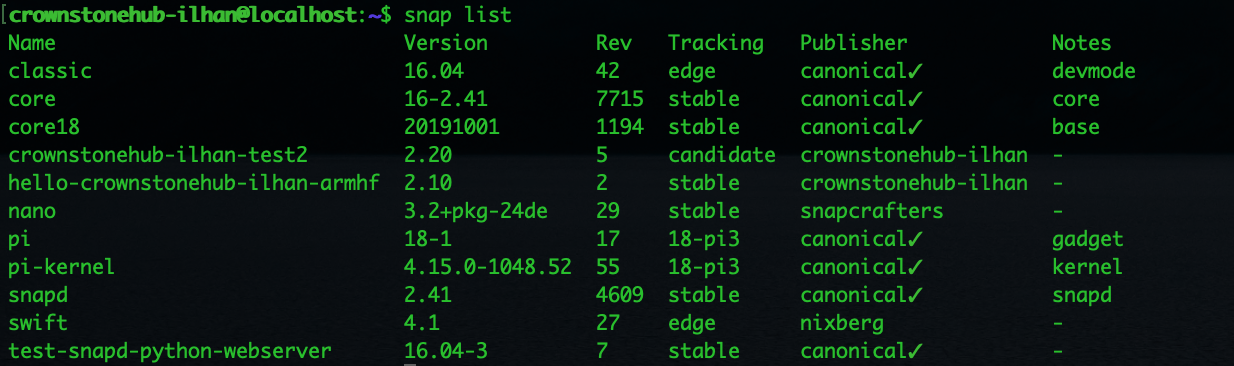
\includegraphics[width=5in]{snapList.png}
	\caption[Optional caption]{snap list}
	\end{figure}
To take a look at the history of the changes you've made enter the following command: 
			\begin{center}				
			"snap changes"
			\end{center}
\label{fig:snapChange}	
	\begin{figure}[H]
	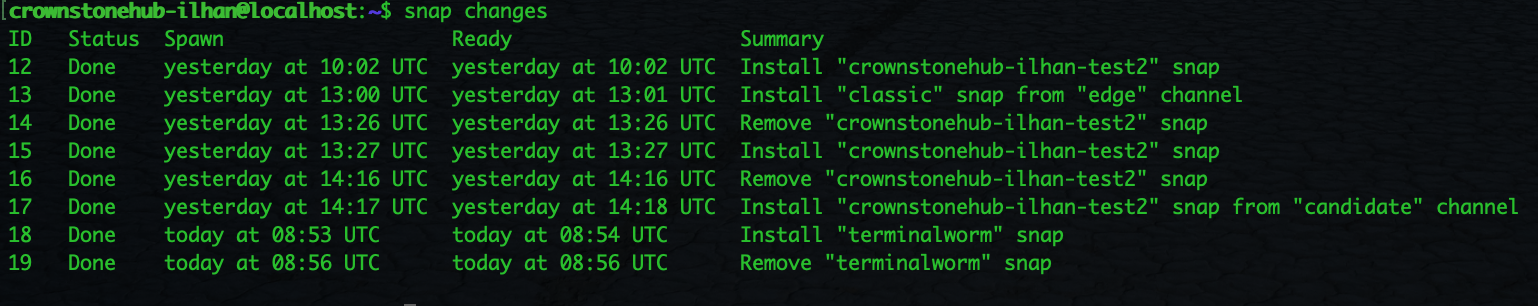
\includegraphics[width=5in]{snapChange.png}
	\caption[Optional caption]{snap change}
	\end{figure}
%-------------------------------------------------------------------------------------------------------------
\cleardoublepage
\subsection{Snap info}\label{sec:info}
If you'd want to run a snap but don't know how you can check the commands of the snap and more information: \\
			\begin{center}				
			"snap info $<snap name>$"
			\end{center}
\label{fig:snapInfo}	
	\begin{figure}[H]
	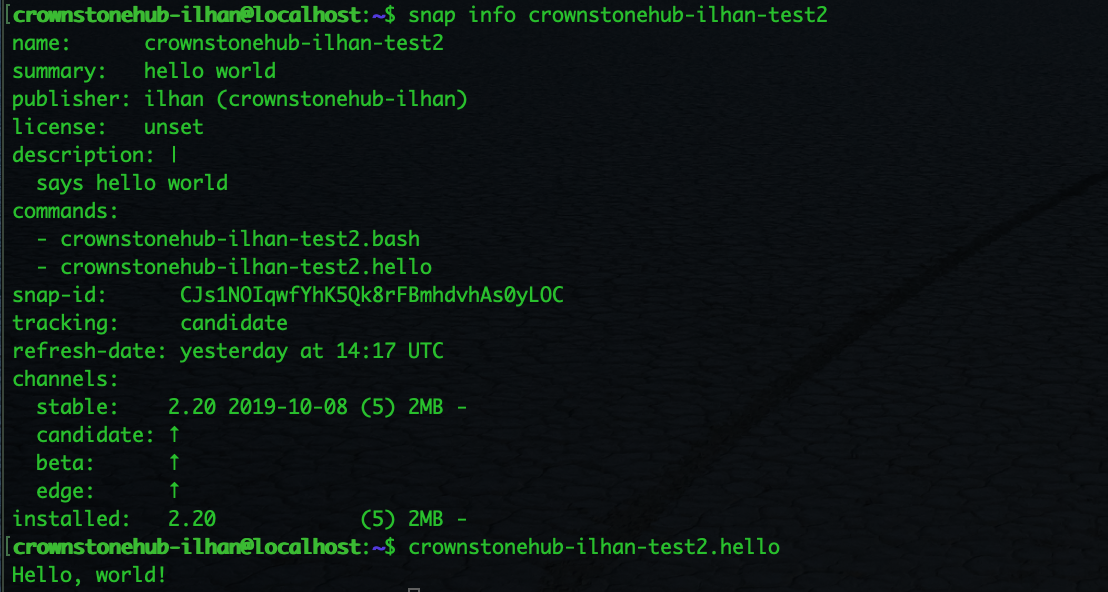
\includegraphics[width=5in]{snapInfo.png}
	\caption[Optional caption]{snap info}
	\end{figure}
	
%-------------------------------------------------------------------------------------------------------------
\subsection{Upgrading and downgrading your snap}\label{sec:refresh}
You could also choose to upgrade or downgrade the snaps you downloaded(of it's possible) to update use:\\
			\begin{center}				
			"sudo snap refresh $<package>$"
			\end{center}
			
To see which snap update is ready to be installed type in: 
			\begin{center}				
			"sudo snap refresh - -list"
			\end{center}
\label{fig:snapRefreshList}	
	\begin{figure}[H]
	
\includegraphics[width=5in]{snapRefreshList.png}
	\caption[Optional caption]{snap refresh list}
	\end{figure}	
	
If for some reason you'd like to undo a update and return to a previous version of the snap use the command: 
			\begin{center}				
			"sudo snap revert $<package>$"
			\end{center}
%-------------------------------------------------------------------------------------------------------------
\cleardoublepage
\subsection{Removing a snap}\label{sec:remove}			
When you're done playing with your snap and feel like you don't need it you can just remove it from your device by using the following line: 
			\begin{center}				
			"sudo snap remove $<package>$"
			\end{center}
\label{fig:snapRemove}	
	\begin{figure}[H]
	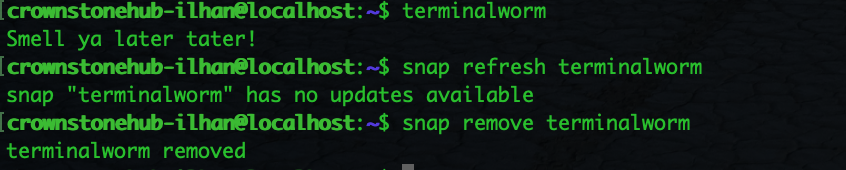
\includegraphics[width=5in]{snapRemove.png}
	\caption[Optional caption]{snap remove}
	\end{figure}	
\bigskip
%-------------------------------------------------------------------------------------------------------------
\subsection{Snap channels}\label{sec:channels}
Snap also has a feature called channels. By default, Snap packages are installed from the ‘stable’ channel. But there are few other channels that give you access to the development version of a program. It’s like switching branches in git, if you are familiar with software development.\\
These channels are:\\
\bigskip
stable: The latest stable release of an application\\
\bigskip
candidate: The release candidate of an application that is reaching the stable version\\
\bigskip
beta: Unstable version that has reached a certain milestone\\
\bigskip
edge: Daily/nightly build of an application under development\\
\bigskip
Needless to say that you should stay on the Stable channel but if you really want to change to another channel, you can use Snap command in the following fashion:\\
			\begin{center}				
			"sudo snap refresh $<package>$ - -channel=$<channel name>$"
			\end{center}
			
Once you changed the channel, your installed package will get updates from that channel. You can switch back to the old channel either by using the refresh command as shown above or simply use the revert command shown above.\\
\cleardoublepage
%
%
%
%-------------------------------------------------------------------------------------------------------------
%
%
\section{Starting the snap}\label{sec:snap}
To start of you have to create a general snaps directory followed bij a working directory for this specific snap project. Using the following commands:
	\begin{center}	
	"mkdir -p ~/ name directory / name snap "\\
	e.g. "mkdir -p ~/mysnaps/hello"\\
	"cd ~mysnaps/hello"\\
	\end{center}
It is from within this hello directory where we will invoke all subsequent commands.\\
Get started by initialising your snap:\\
	\begin{center}	
	"snapcraft init"\\ 
	\end{center}
This created a snapcraft.yaml in which you declare how the snap is built and which properties it
exposes to the user. We will edit this later.\\
The directory structure looks like this:\\
mysnaps/\\
  hello/\\
    snap/\\
      snapcraft.yaml\\
    	 NOTE:\\
	Any future snap would be put in its own directory under mysnaps.\\
\label{fig:step2}
	\begin{figure}[H]
	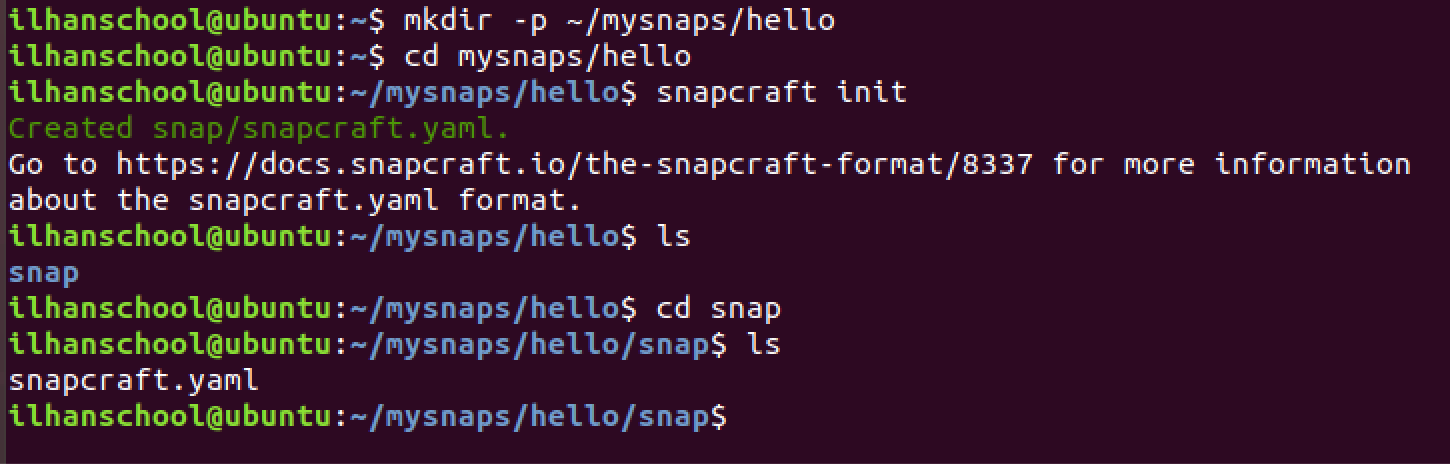
\includegraphics[width=5in]{step2.png}
	\caption[Optional caption]{snapcraft directory}
	\end{figure}
	
	\cleardoublepage
%
%
%
%
%------------------------------------------------------------------------------------------------------
%
%
\subsection{describing the snap}\label{describe snap}
	Let's take a look at the top part of your snapcraft.yaml file. Use "nano snapcraft.yaml" while you're in the ~mysnaps/hello/snap directory. It should look 
	somewhat as shown below:\\

	\begin{figure}[H]

	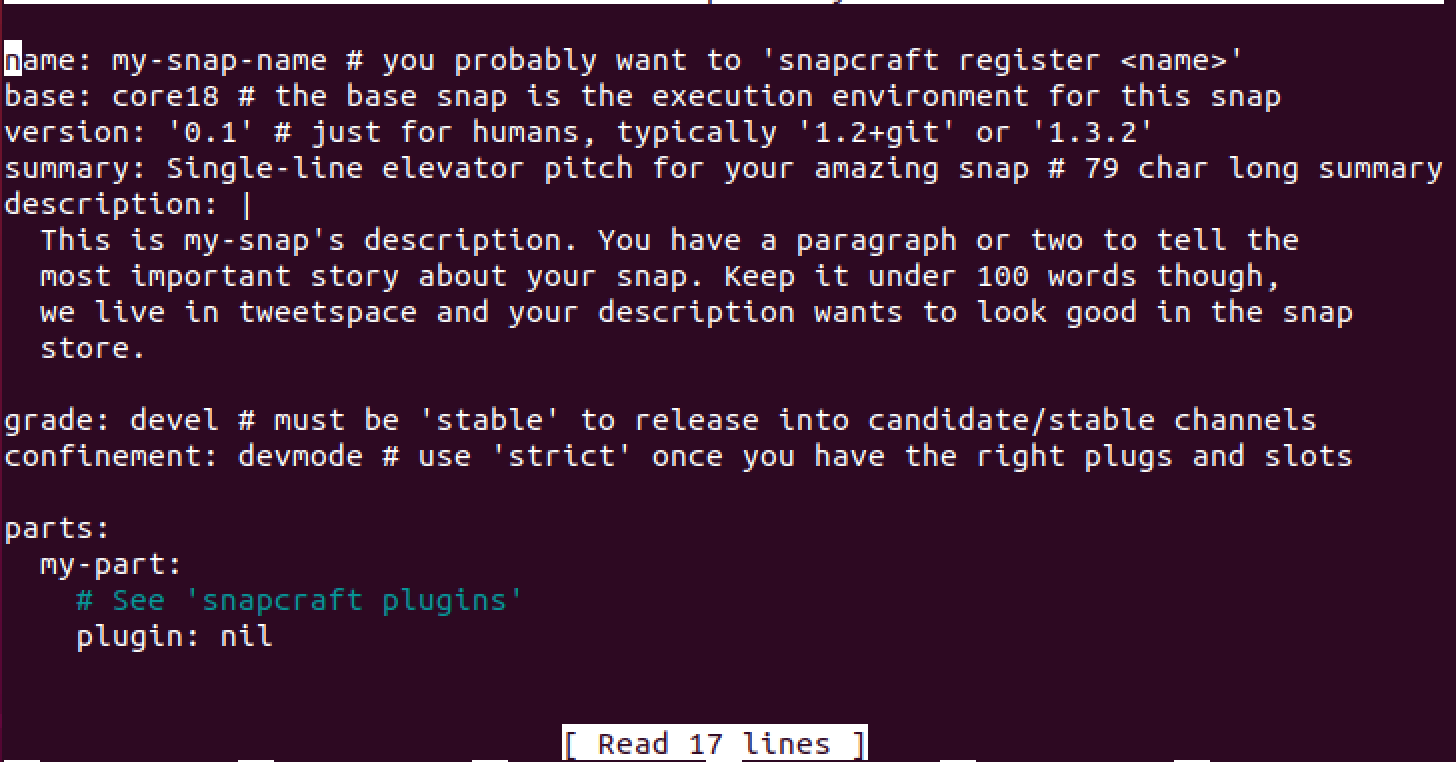
\includegraphics[width=5in]{step17.png}
	\caption[Optional caption]{default text}
	\label{fig:step17}
	\end{figure}
	
\begin{flushleft}	
This part of snapcraft.yaml is mandatory and is basic metadata for the snap.
Let's go through this line by line:\\
[5mm]
NAME: The name of the snap.\\
[5mm]
VERSION: The current version of the snap. This is just a human readable string. All snap
uploads will get an incremental snap revision, which is independent from this version. It's
separated so that you can upload multiple times the same snap for the same architecture with
the same version. See it as a string that indicates to your user the current version, like
"stable", "2.0", etc.\\
[5mm]
SUMMARY: A short, one-line summary or tag-line for your snap.\\
[5mm]
DESCRIPTION: A longer description of the snap. It can span over multiple lines if prefixed
with the ‘|' character.\\
[5 mm]

GRADE: Can be used by the publisher to indicate the quality confidence in the build. The
store will prevent publishing ‘devel' grade builds to the ‘stable' channel.\\
\cleardoublepage

CONFINEMENT: Can be either ‘devmode', ‘strict', or ‘classic'. A newly-developed snap should start out
in devmode. Security requirements can get in the way during development and ‘devmode' eases
these requirements. Security aspects like confinement can be addressed once the snap is
working. If there are technical issues that obstruct the confinement of a snap, it may also be developed and released using classic confinement. Classic imposes no additional restrictions and effectively grants device ownership to the snap. Consequently, snaps using classic confinement require a manual review before being released to the store (see Classic confinement review process for further details).However, in this tutorial we will only focus on devmode and strict confinement.
\end{flushleft}	
\cleardoublepage
%
%
%------------------------------------------------------------------------------------------------------
%
%
\section{Customisation}\label{sec:customisation}
That's it for the basics, now you're going to customise your snap.\\
Use the command "nano snapcraft.yaml" to edit the text to make snapcraft.yaml look like this:\\
\label{fig:step5}

	\begin{figure}[H]
	\includegraphics[width=5in]{step5.png}
	\caption[Optional caption]{snapcraft.yaml 1.0}
	\end{figure}
\begin{flushleft}	

Note:\\
- Make sure you set a space after the colon(":").\\
- Use the spacebar instead of tabs to set the outline\\
- Version information is for snap user consumption only, and has no effect on snap updates. It's defined within quotes, ('2.10'), because it needs to be a YAML string rather than a floating-point number. Using a string allows for non-numeric version details, such as ‘myfirstversion' or ‘2.3-git'.
\cleardoublepage
%
%
%------------------------------------------------------------------------------------------------------
%
%
%
\subsection{Adding a part}\label{sec:adding part}
A snap can consist of multiple parts. Here are a few examples of this:

Snaps with separate logical parts, e.g. a server snap, which contains a web server, a database
and the application itself or a game which ships the game engine and game data for three
different games, each one being defined in its own part.
Snaps with parts which come from different locations.
Parts which are built in a different way.
Our hello snap will be nice and simple. It will consist of only one part for now. In the
following pages we are going to gradually extend it.\\

\bigskip% skip a line
Two must-haves for every part are the ‘source' and ‘plugin' definition. Think of these as the
"what" and the "how", respectively. As source you can, for example, pick a source repository (like
git), a tarball, or a local directory. Snapcraft supports many plugins, allowing you to build
a wide variety of project types (e.g. autotools, cmake, go, maven, nodejs, python2, python3).\\
To build hello the snapcarft.yaml file needs to look like this: \pageref{fig:step5}\\
\bigskip 
To build the snap use the command: \\
		\begin{center}	
			"snapcraft"\\ 
			\end{center}
now you should get this:
\label{fig:step4}
	\begin{figure}[H]
	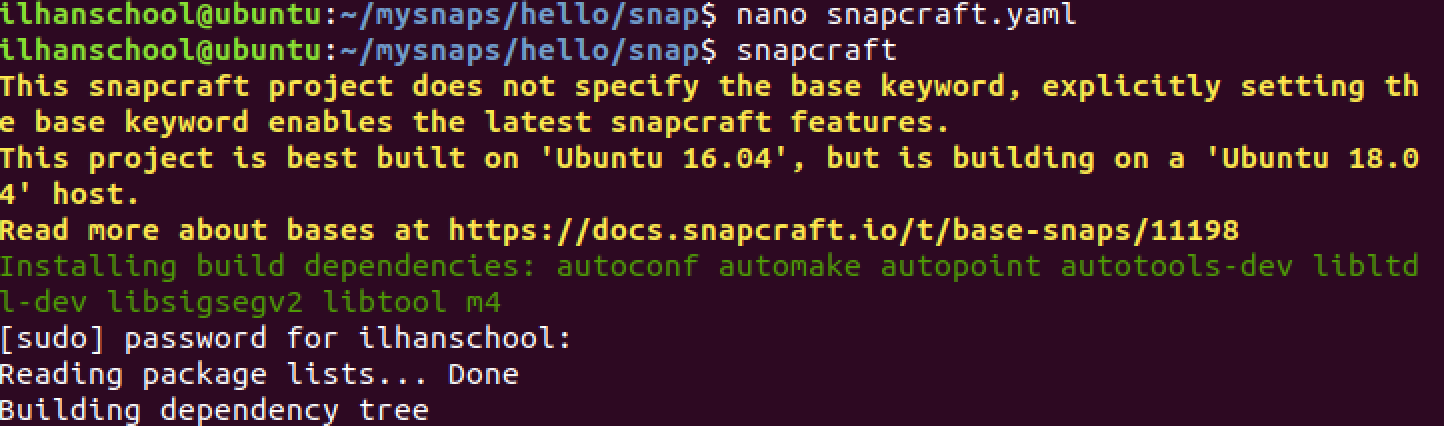
\includegraphics[width=5in]{step4.png}
	\caption[Optional caption]{snapcraft command}
	\end{figure}
	 
\label{fig:step6}	
	\begin{figure}[H]
	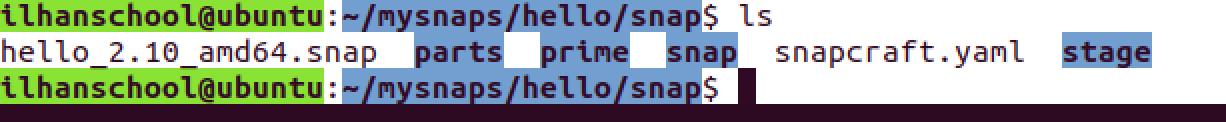
\includegraphics[width=5in]{step6.png}
	\caption[Optional caption]{the snap directory after the first build}
	\end{figure}
\cleardoublepage
Next install the snap you've just build: 
			\begin{center}	
		"sudo snap install - -devmode $<name|_snap>$ \pageref{fig:step6}" 
			\end{center}
Like so:
	\label{fig:step7}
	\begin{figure}[H]
	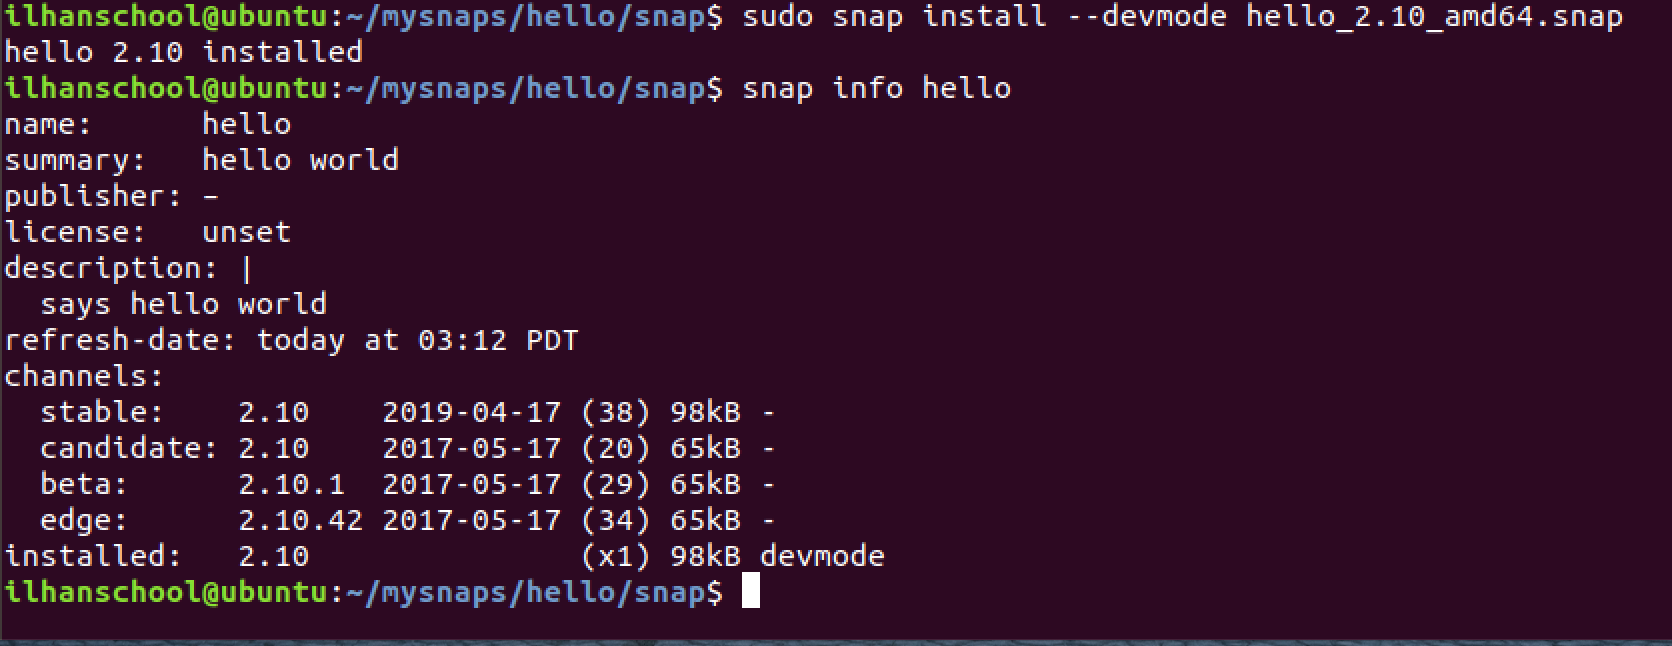
\includegraphics[width=5in]{step7.png}
	\caption[Optional caption]{snap install 1}
	\end{figure}
Snap list shows the information given in the snapcraft.yaml file.
Now we're able to build the snap but it doesn't have any commands to run. We'll need to add another part to the snapcraft.yaml\\
\cleardoublepage 

Open the snapcraft.yaml file and make it look like this to add an command to run:
\label{fig:step8}	
	\begin{figure}[H]
	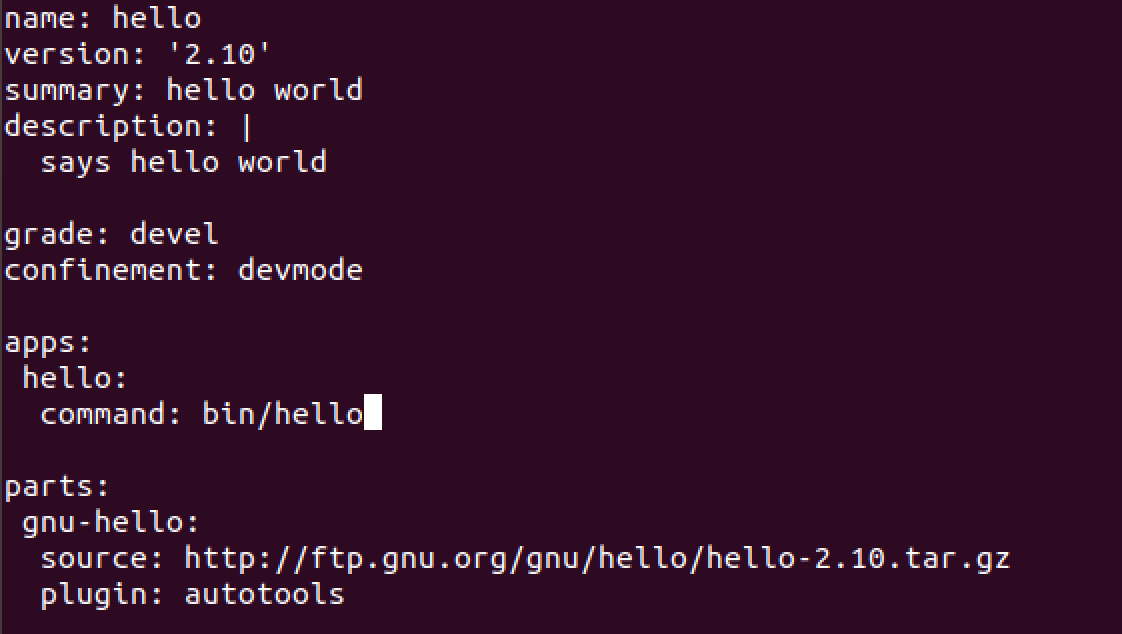
\includegraphics[width=5in]{step8.png}
	\caption[Optional caption]{snapcraft.yaml 2.0}
	\end{figure}
Now the snap can finally be build. Use the following commands: 
			\begin{center}	
			"snapcraft prime"\\ 
			\end{center}
			
What we did was tell snapcraft to run the build up until the "prime" step. That is, we are
omitting the "pack" step (see lower down for an explanation of each step in a snapcraft
lifecycle \pageref{ref:snaplife}). What this invocation gives therefore are the unpacked contents of a snap.\\

We can then provide this content to "snap try":
			\begin{center}	
			"sudo snap try - -devmode prime"\\ 
			\end{center}
\label{fig:step9}	
	\begin{figure}[H]
	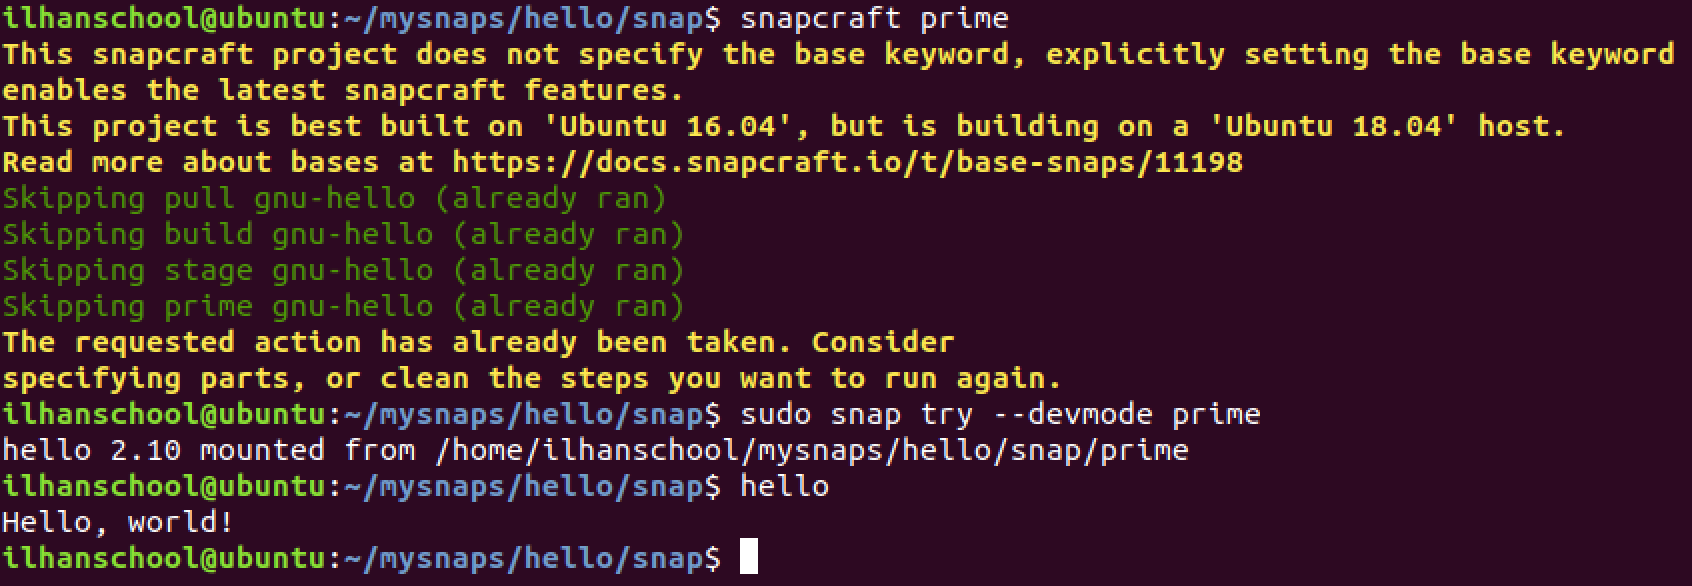
\includegraphics[width=5in]{step9.png}
	\caption[Optional caption]{snap try output}
	\end{figure}

Note:\label{ref:snaplife}\\ 
The different steps of the snapcraft lifecycle are: "pull" (download source for all parts), "build", "stage"\\
(consolidate installed files of all parts), "prime" (distill down to just the desired files), and
"pack" (create a snap out of the prime/ directory). Each step depends on the successful completion
of the previous one.\\
\bigskip
Things should be working now, test it by using the following:
			\begin{center}	
			"snapcraft prime"\\ 
			\end{center}

\label{fig:step18}	
	\begin{figure}[H]
	
\includegraphics[width=5in]{step18.png}
	\caption[Optional caption]{hello output}
	\end{figure}
Important:\\
If hello does not run and you get the error cannot change current working directory to the
original directory: No such file or directory then most likely you are developing the snap in a
directory other than your home directory. An example of a directory that would generate this error,
is the /tmp/ directory. Fix it by uninstalling the snap with sudo snap remove hello and
starting over.					
\end{flushleft}
\cleardoublepage
%
%
%------------------------------------------------------------------------------------------------------
%
%
\subsection{Adding another part}\label{sec:adding another part}
\begin{flushleft}
In order to make your snap do more than one thing you should add more parts to it so you can run more than 1 command. Open de snapcraft.yaml and make it look like this: 
\label{fig:step10}	
	\begin{figure}[H]
	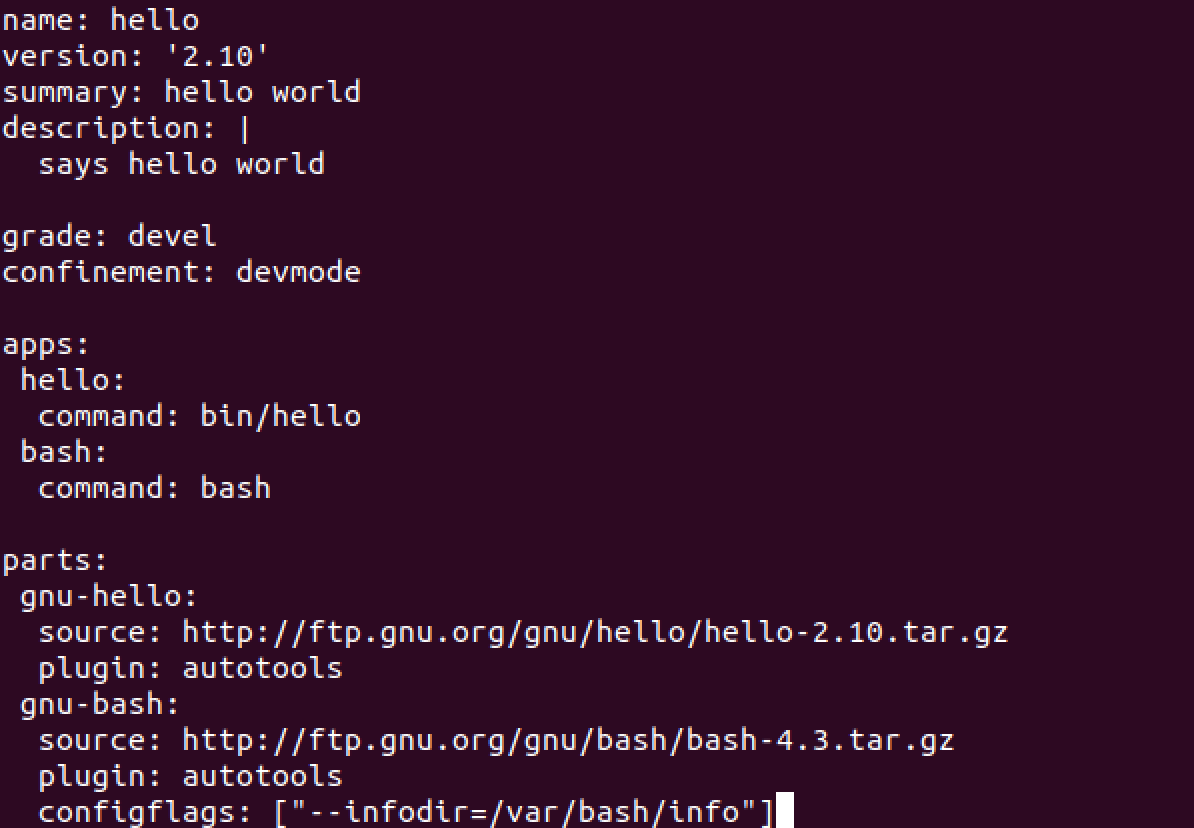
\includegraphics[width=5in]{step10.png}
	\caption[Optional caption]{snapcraft.yaml 3.0}
	\end{figure}
Make sure you add the last line to avoid this error: \\
"Failed to stage: Parts 'gnu-bash' and 'gnu-hello' have the following files, but with different contents:
    share/info/dir"\\
    What does this mean? Both our gnu-hello and gnu-bash parts want to ship a version of
share/info/dir with differing contents. The two most common ways to rectify this kind of problem
are:\\

\bigskip
- Instruct only one of the two parts to place content in this directory. We can also tell both
to supress the content. Which solution depends on the necessity of said content. Either is
achieved by influencing the ‘snap' and ‘stage' steps.\\
- Change the directory location for one of the two parts.\\
\bigskip
By adding the last line in de snapcraft.yaml you avoid this error by changing the directory of the new part.
\cleardoublepage

%
%
%
%------------------------------------------------------------------------------------------------------
%
%
\cleardoublepage
\section{Remove devmode}\label{sec:remove dev}
One last thing you might want to do before the snap is ready for wider consumption is to remove the
devmode status.\\
\bigskip
Important:\\
Users of snaps using devmode, will need to pass --devmode during the installation, so they
explicitly agree to trust you and your snap. Another benefit of removing devmode is that you will
be able to ship your snap on the ‘stable' or ‘candidate' channels (you can only release to the
other channels, like ‘beta' or ‘edge' as your snap is less trusted) and users will be able to
search for it using snap find.\\

\bigskip 
For this to be declared in your snap, let's set confinement to "strict" in the snapcraft.yaml. 

\label{fig:step13}	
	\begin{figure}[H]
	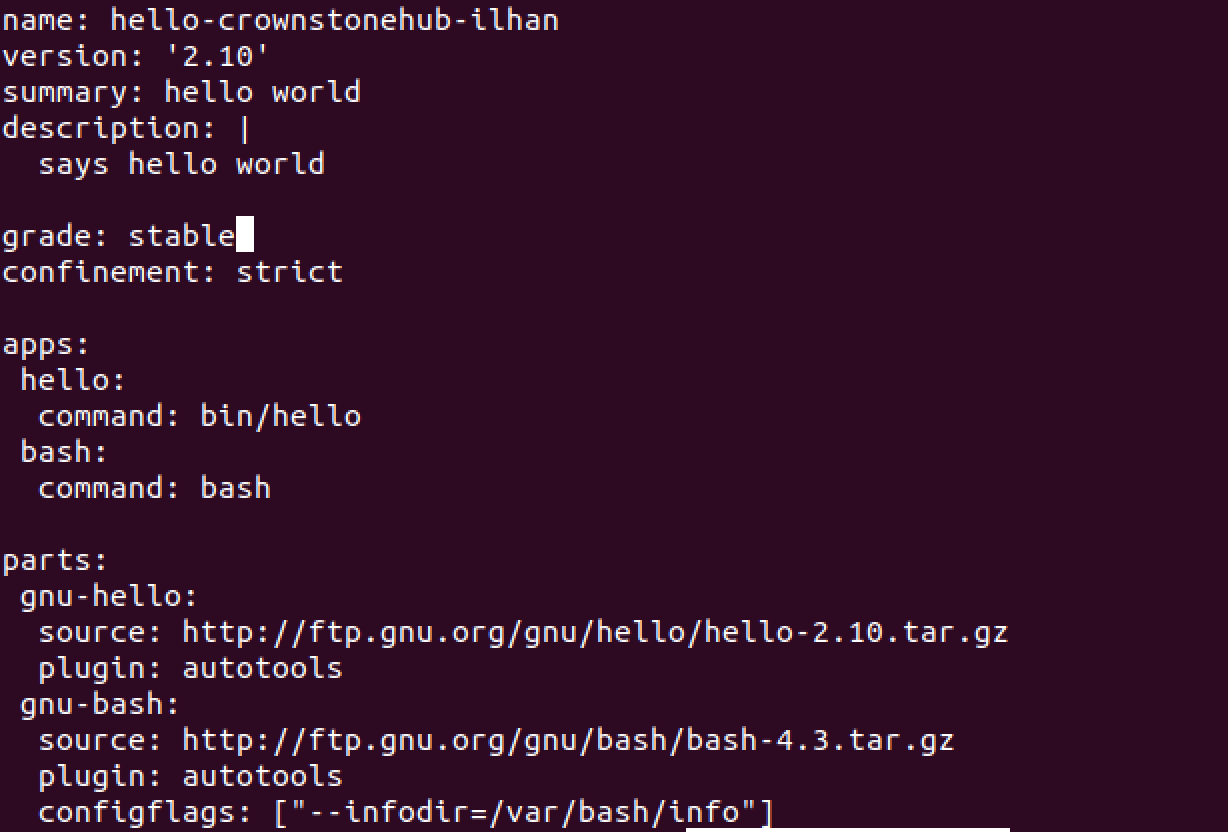
\includegraphics[width=5in]{step13.png}
	\caption[Optional caption]{snapcraft.yaml 4.0}
	\end{figure}
\cleardoublepage

\label{fig:step12}	
	\begin{figure}[H]
	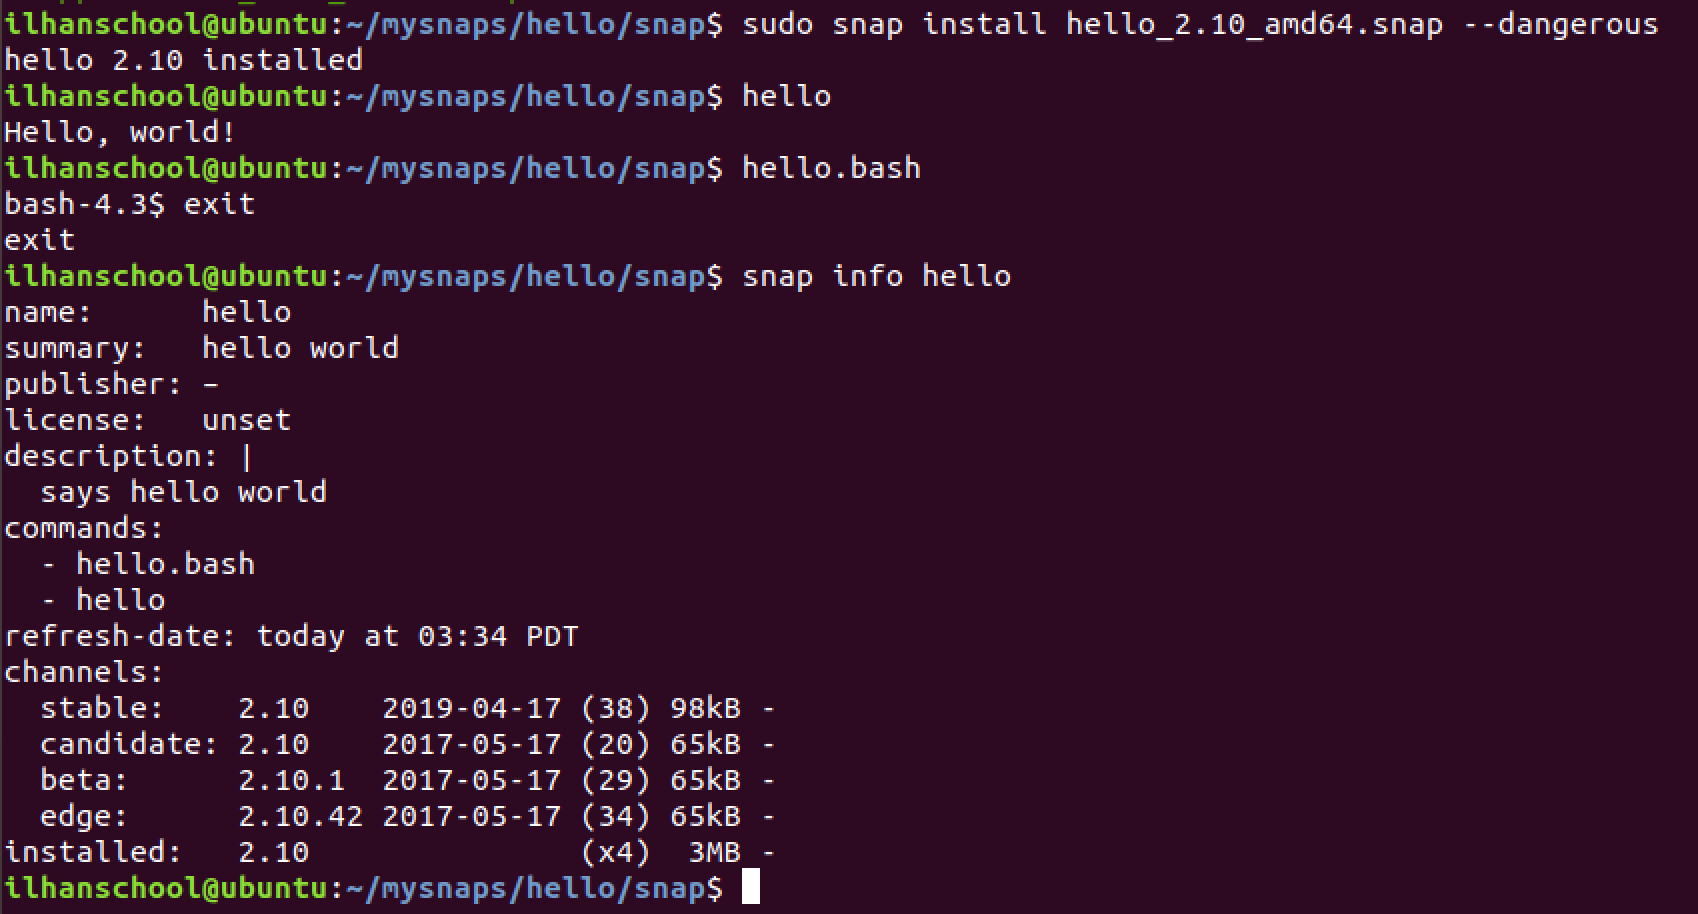
\includegraphics[width=5in]{step12.png}
	\caption[Optional caption]{- -dangerous}
	\end{figure}
If you don't add the - -dangerous in the line the it will not install, because the snap isn't signed by the Snap Store yet. With the - -dangerous added at the end of the line it can install without being signed by the Snap Store. Now try  the commands "hello" and "hello.bash" as shown in the figure above. 
\cleardoublepage
%
%
%
%------------------------------------------------------------------------------------------------------
%
%
\section{Push to the store}\label{sec:push2store}
For this part you'll need an Ubuntu SSO account to proceed. If you have an Ubuntu SSO account go to the snapcraft dashboard: {https://dashboard.snapcraft.io/}\\
This is the place to manage all the snaps you've build and published.
At the top of the webpage you'll see an add snap button click it and you'll be able to choose a name for the snap you've made. 
\label{fig:step19}	
	\begin{figure}[H]
	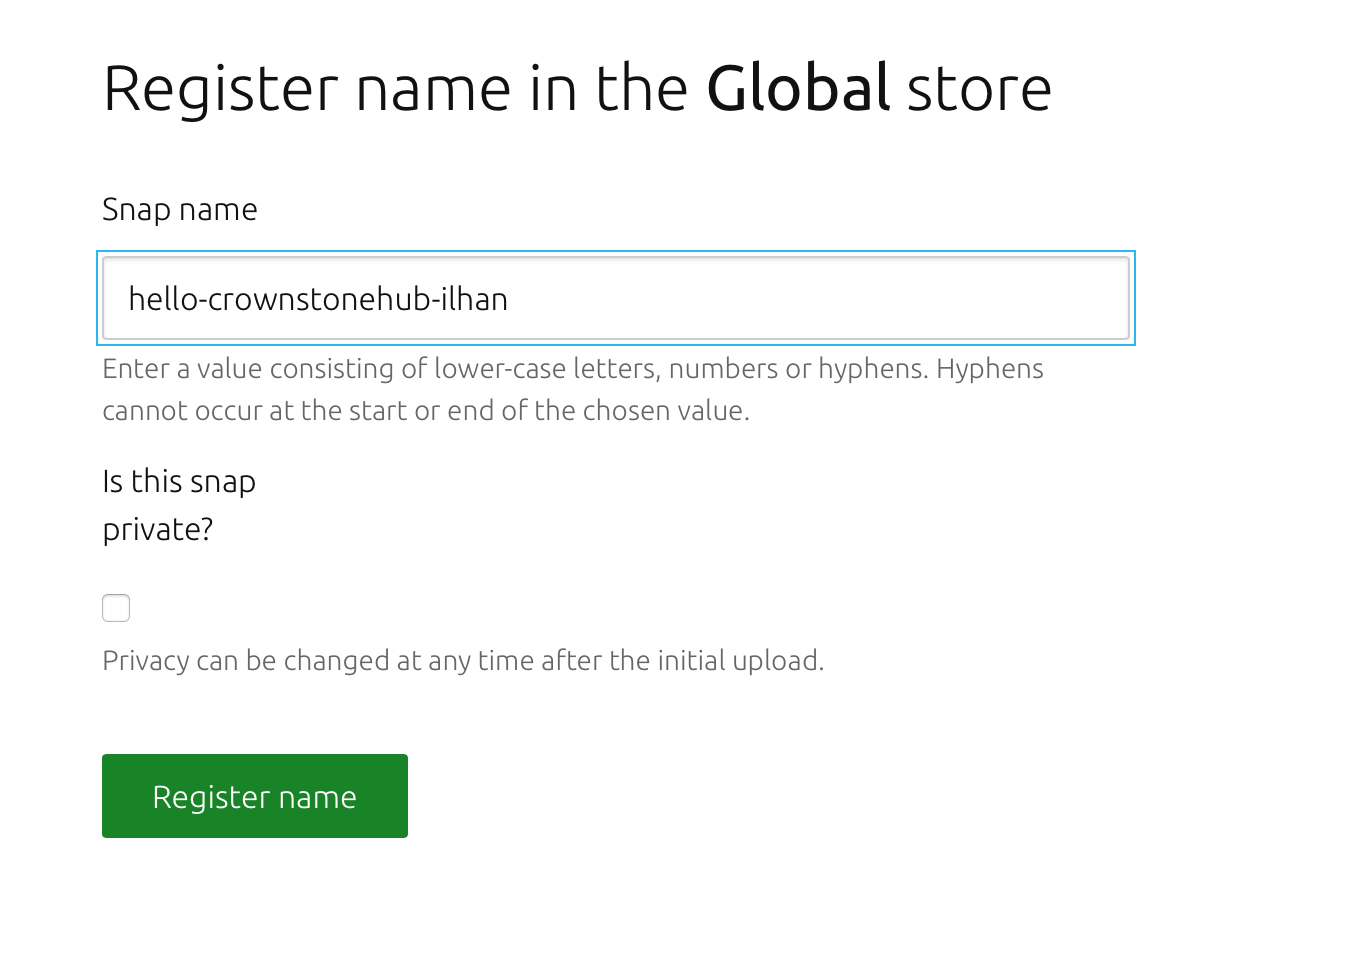
\includegraphics[width=5in]{step19.png}
	\caption[Optional caption]{snap name}
	\end{figure}
Click register name.

\label{fig:step20}	
	\begin{figure}[H]
	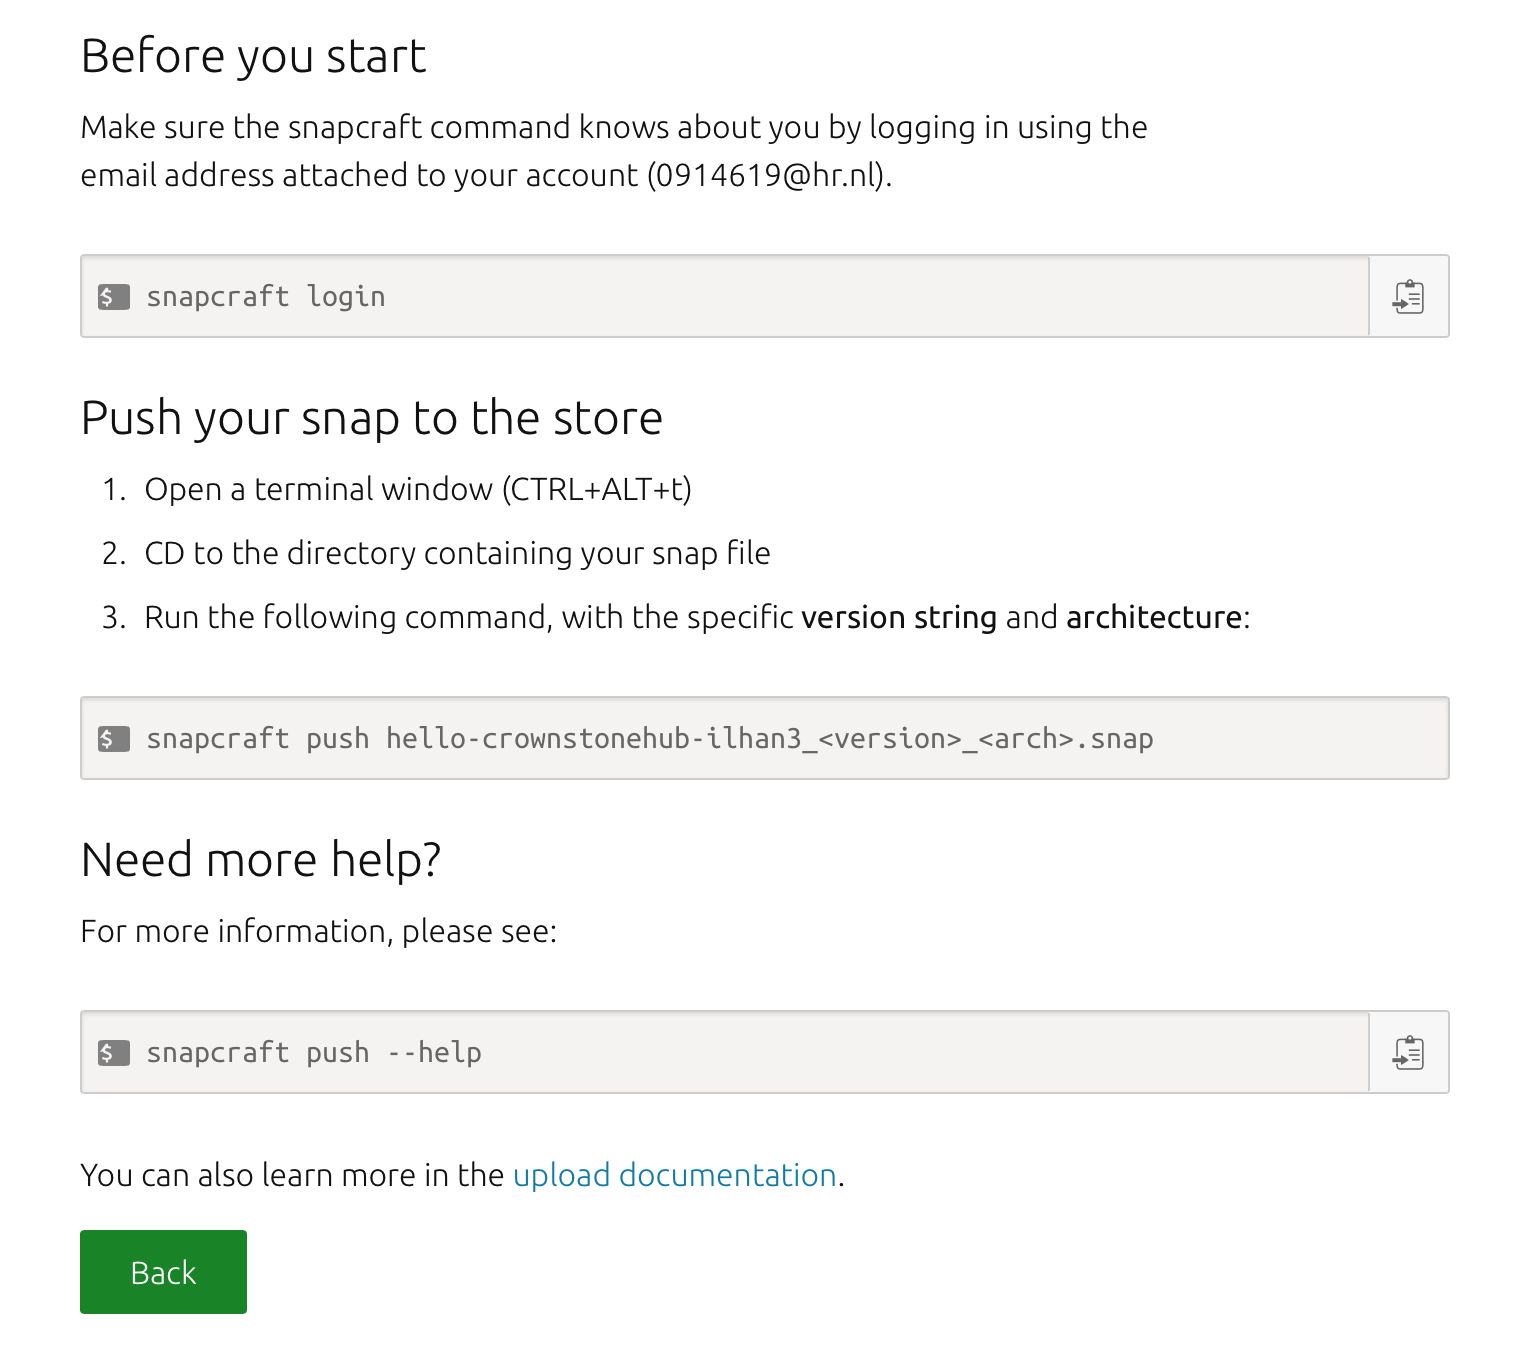
\includegraphics[width=5in]{step20.png}
	\caption[Optional caption]{snap name 2.0}
	\end{figure}

If you don't want to be on a desktop and stay in your comfortable terminal.The next steps would need to be executed on the terminal:
			\begin{center}	
			"snapcraft login"\\
			Enter your ubuntu SSO email and password\\
			 "snapcraft register $<some name>$ "\\
			\end{center}
			\cleardoublepage
Now you'll see the following:
\label{fig:step15}	
	\begin{figure}[H]
	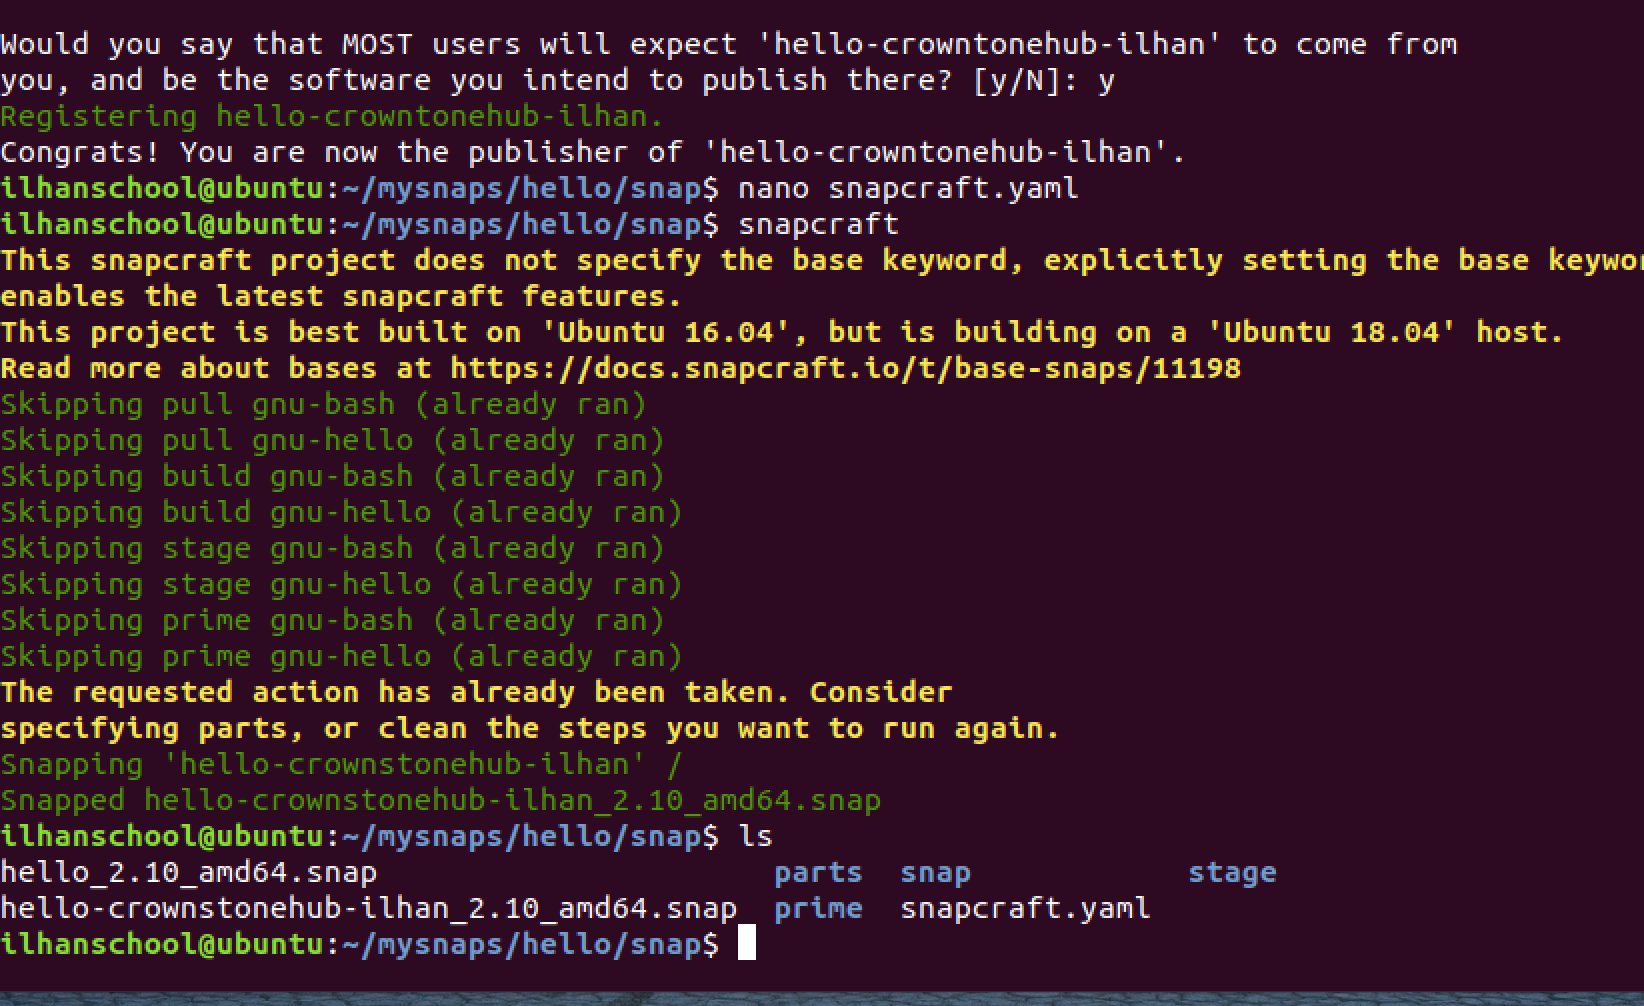
\includegraphics[width=5in]{step15.png}
	\caption[Optional caption]{snap publish}
	\end{figure}
You'll be asked if the name you chose is the right one if so answer  "y".	
The next thing to do is to change the name in your snapcraft.yaml to the name you've just accepted. and change the grade from strict to stable like: \pageref{fig:step13}
\bigskip
Rebuild the snap using the command as shown in figure above:
			\begin{center}	
			"snapcraft"\\ 
			\end{center}

Now you can release the snap on the 'candidate' channel for now:
			\begin{center}	
			"snapcraft push $<namesnap>\_<version>\_<architecture>$.snap - -release=candidate "\\ 
 "name\_version\_architecture.snap" \\
			\end{center}
\cleardoublepage
 Now you can release the snap on the 'candidate' channel for now:
			\begin{center}	
			"sudo snap install $<name>$ - -channel=candidate"
			\end{center}

In order to make your snap available in the store run this commandline:
			\begin{center}	
			"snapcraft release $<namesnap> <revision> <channel>$\\
			\end{center}
like so:
\label{fig:step16}	
	\begin{figure}[H]
	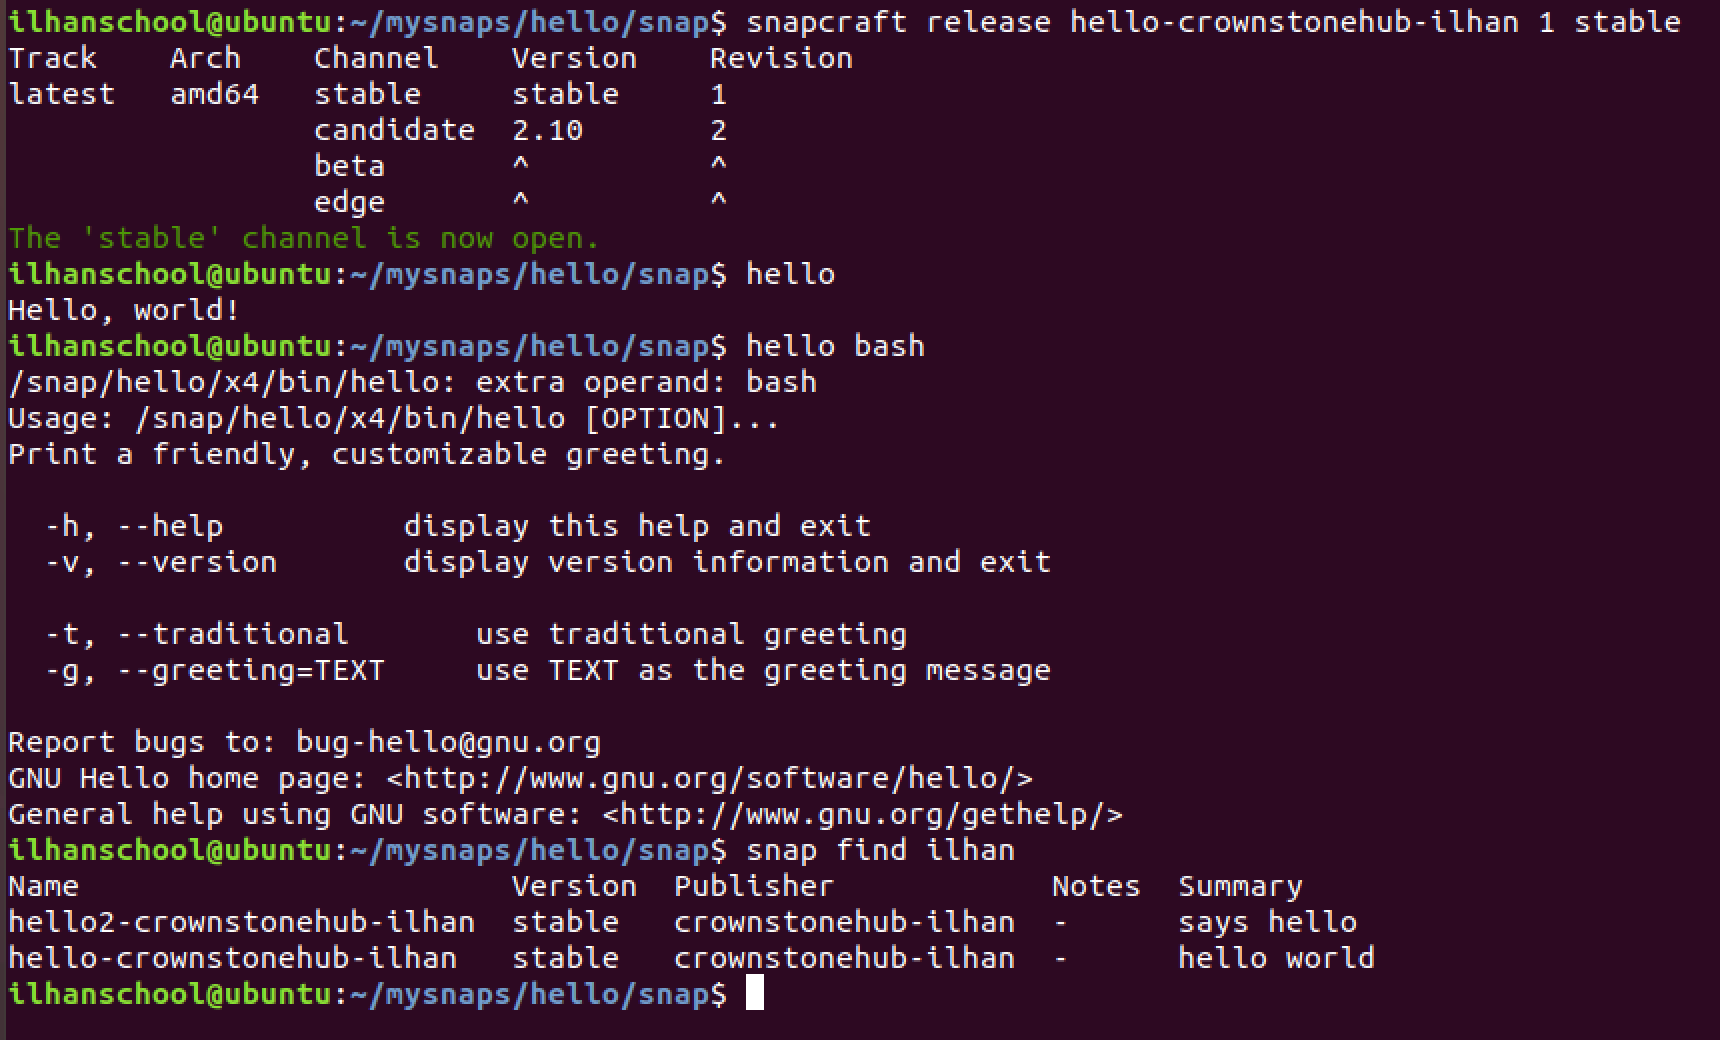
\includegraphics[width=5in]{step16.png}
	\caption[Optional caption]{to the store}
	\end{figure}
With the other commands shown in the figure you'll be able to find out of you downloaded the snap. 
\cleardoublepage
%
%
%
%
%
%
%-------------------------------------------------------------------------------------------------------------
%		hier moet je nog over lezen over het over zetten van amd64 naar armhf
%
%
%
\section{Crosscompile amd64 to armhf}\label{sec:crosscompile}

The biggest issue I faced while making a snap for a raspberryPi on an linux computer was the fact that I couldn't find the snap in the store while i was using ubuntu core on the raspberryPi.\\
One way to make the snap work on the raspberryPi is to actually build it on the raspberry. In order to do this you'd have to install a couple of other additional snaps.
\bigskip

NOTE: \\
You'd only need 1 raspberryPi to build it and push it to the snap store from here you can download the snap on any other raspberry with ubuntu (core) and not have the additional snaps installed.
%-------------------------------------------------------------------------------------------------------------
\subsection{Building on the raspberryPi}\label{sec:rPibuild}
The first way I fixed the snap on raspberry issue is to build the snap on a Pi. I had to install a couple of additional snaps to make this work. We'll need to edit files and run snapcraft. Snapcraft can not be installed on ubuntu core! Luckily you can install a traditional ubuntu mode called "classic". So we're going to install classic first. To do so run:\\
			\begin{center}	
			"sudo snap install classic --edge --devmode"\\ 
			\end{center}
To run classic and install snaps or packages that can't be installed on ubuntu core run:\\
			\begin{center}	
			"sudo classic"\\ 
			\end{center}
			
We also need to edit files because of this we'll install nano:\\
			\begin{center}	
			"sudo apt-get install nano"\\ 
			\end{center}
The last thing to install is snapcraft. (\pageref{sec:installation})\\
Now that everything is installed we can start making the snap. Make a new directory (\pageref{sec:snap}) and make the snapcraft.yaml file like in the tutorial above. When you're done with the yaml file run the command snapcraft(\pageref{fig:step4}) and push the snap to the store (\pageref{sec:push2store}). When the snap is pushed into the store successfully  you can download the snap on other amrhf devices without any other snaps. It will look like this (\pageref{fig:snapInfo}).\\
\cleardoublepage
%-------------------------------------------------------------------------------------------------------------
\subsection{Convert with linux desktop}\label{sec:linuxBuild}

I've tried a snap builder by Launchpad
at the moment this page is under construction because i don't have this bit fully working as need be
%-------------------------------------------------------------------------------------------------------------
\end{flushleft}
\end{flushleft}
\end {document}

%
%https://tutorials.ubuntu.com/tutorial/create-your-first-snap#4
%https://itsfoss.com/use-snap-packages-ubuntu-16-04/
%https://viteinfinite.com/2017/02/swift-on-the-raspberry-pi-part-1/
%
%




